%!TEX root = ./ERL Industrial Robots.tex


%--------------------------------------------------------------------
%--------------------------------------------------------------------
\subsection{Manipulation Place Functionality}
\label{ssec:ManipulationPlace}

%--------------------------------------------------------------------
\subsubsection{Functionality Description}
\label{sssec:ManipulationPlaceDescription}

This functionality benchmark assesses the robot's capability of placing different objects. 
An object from a known set of possible objects is presented in the test for the robot to be placed.
After grasping the object, the robot needs to perform the placing motion, lift the object and place the object in a particular container/box.


\begin{figure}[htb]
	\begin{center}
	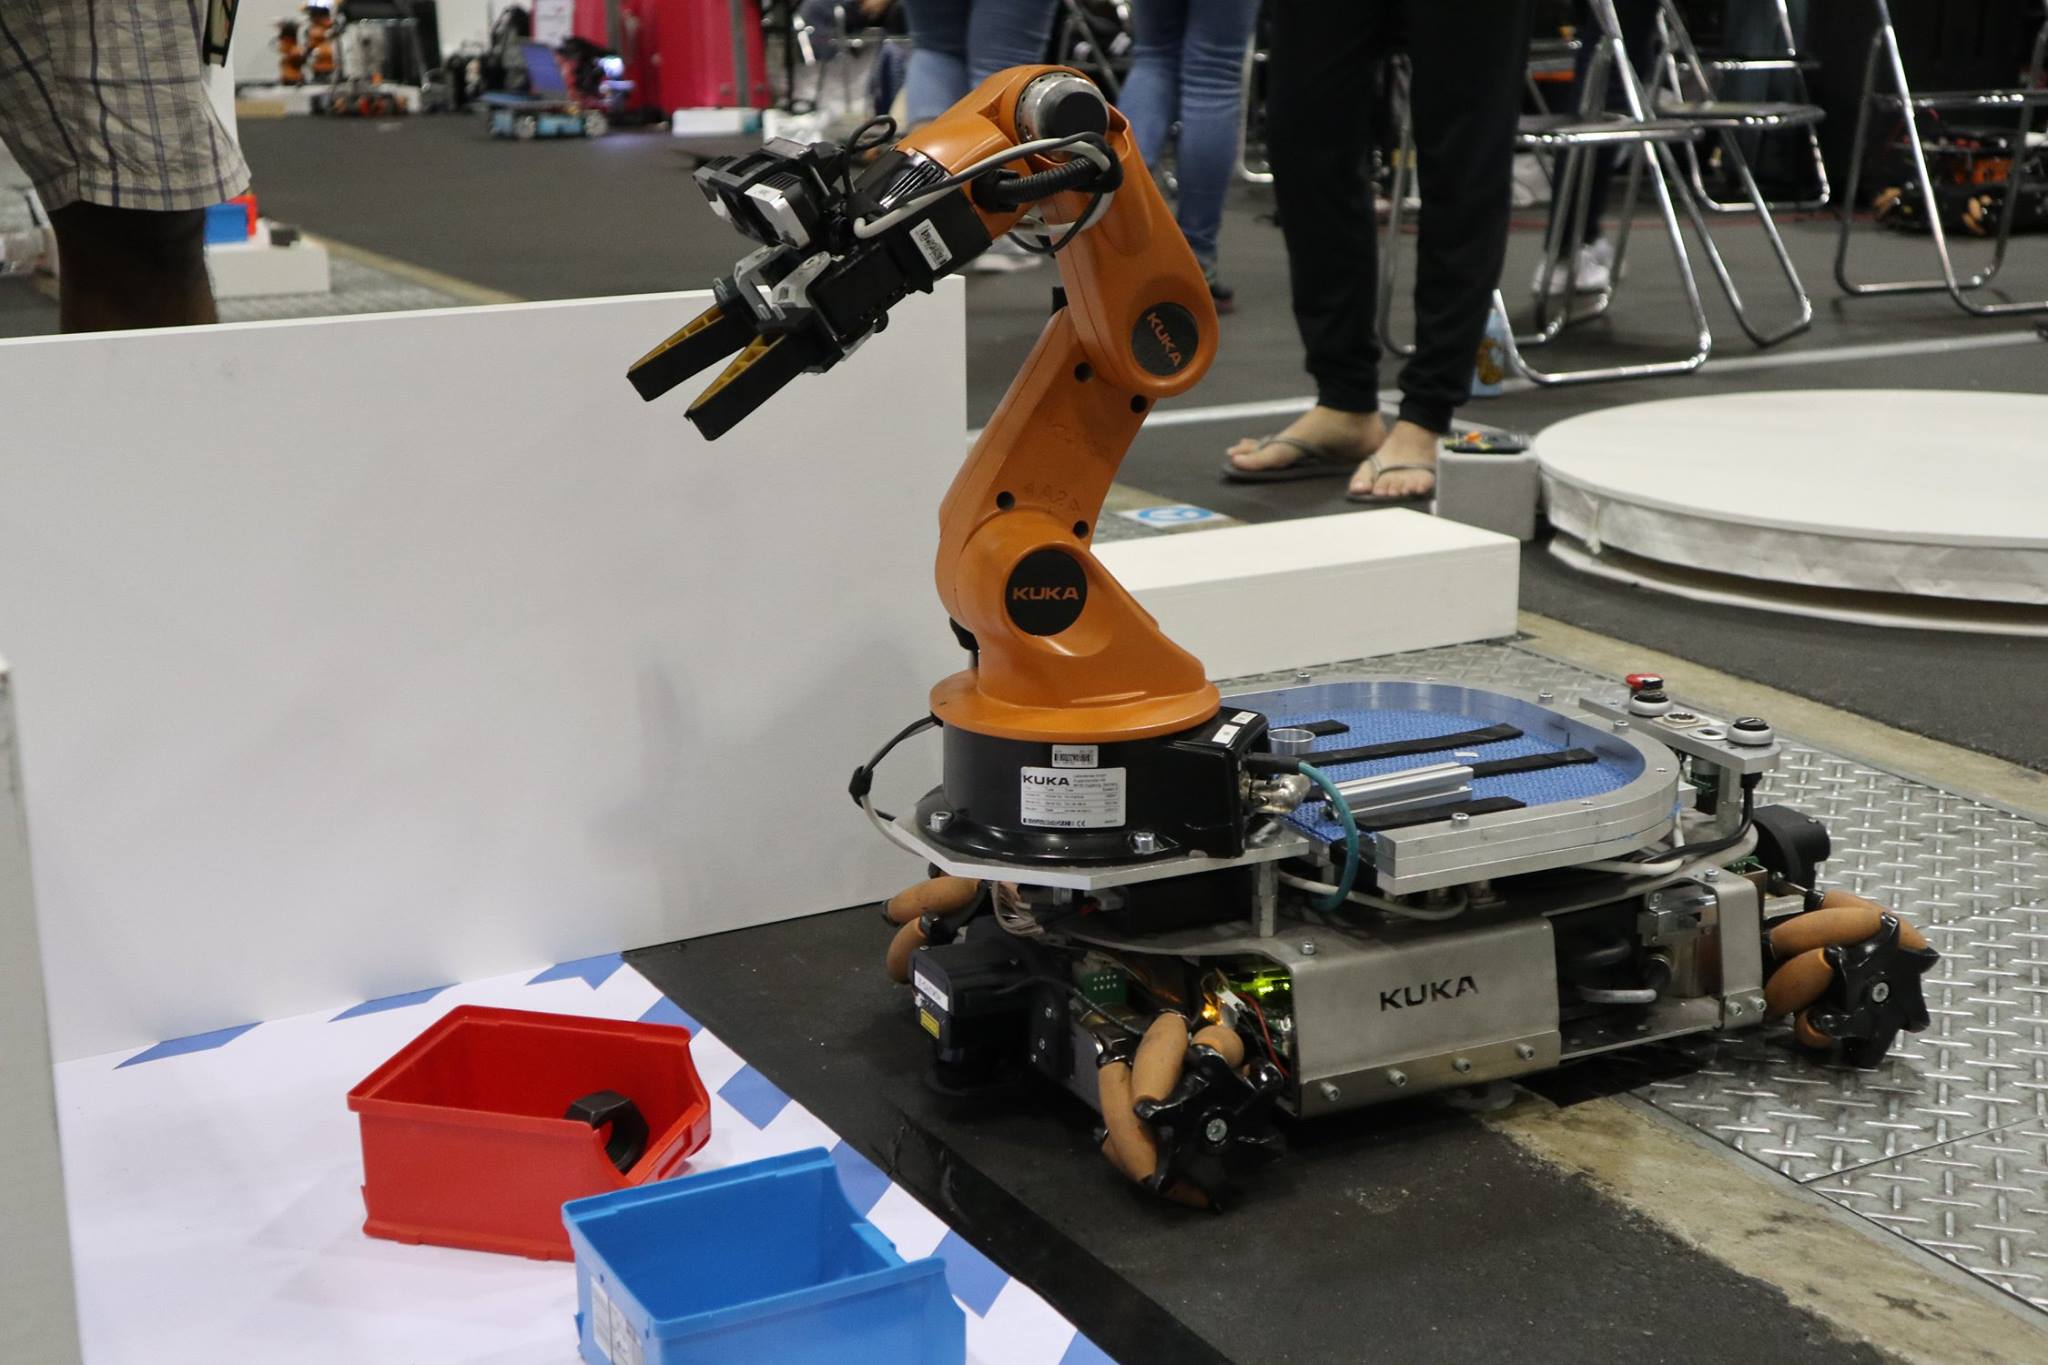
\includegraphics[width=0.45\textwidth]{./fig/FBM/atwork/place_object.jpg}
			\label{fig:MarkerSetEndEffectorWithFrame}
	\caption{Manipulation Place Functionality.}
		\label{fig:ManipulationPlace} 
	\end{center}
\end{figure}
%--------------------------------------------------------------------
\subsubsection{Feature Variation}
\label{sssec:FBMManipulationPlaceVariation}

The objects used in the benchmark will be selected from the list of parts to manipulate as presented in Section \ref{ssec:Objects}.
Additionally, the precise position of the object placement differes in each test.
%--------------------------------------------------------------------
\subsubsection{Input Provided}
\label{sssec:FBMManipulationPlaceInput}

The team will be provided with the following information:
\begin{itemize}
	\item The list of possible objects used in the functionality benchmark.
	\item Possible placement of each object used in the functionality benchmark.
\end{itemize}

%--------------------------------------------------------------------
\subsubsection{Expected Robot Behaviour or Output}
\label{sssec:FBMManipulationPlaceOutput}

The robot is placed in front of the test area (a planar surface).
One object will be placed on the robot or in its gripper.
The robot now has to look the test area for any container to be placed.
The robot performs the placing motion of the object and places the object in particular container in front of it.
After placement it notifies the CFH.



%--------------------------------------------------------------------
\subsubsection{Procedures and Rules}
\label{sssec:FBMManipulationPlaceProcedures}

The maximum time allowed for one functionality run is 4 minutes (30 seconds for preparation and 210 seconds for execution). A run consists of (1) a preparation phase where the robot is going to its initial configuration and  grasp object and (2) an execution phase in which the robot detects, localizes, recognizes and manipulates one object.

\begin{description}
\item[Step 1] An object of known class and known instance will be placed on the robot.
\item[Step 2] The robot must scan the test area and find a container.
\item[Step 3] The robot must place the object inside the container and notify that placing has occurred.
\item[Step 5] The preceding steps are repeated with five different objects.
\end{description} 


\subsubsection{Communication with CFH}
\label{sssec:FBMManipulationPlaceCommCFH}

For this functionality benchmark the robot does not have to control any networked device in the environment. Only the communication as described below is necessary:

\begin{description}
\item[Step 1] The robot sends a \textbf{BeaconSignal} message at least every second.
\item[Step 2] The robot waits for a \textbf{BenchmarkState} message. It starts the preparation procedure when the \emph{phase} field is equal to PREPARATION and the \emph{state} field is equal to RUNNING.
\item[Step 3] As soon as the robot finishes the preparation phase, it sends a message of type \textbf{BenchmarkFeedback} to the CFH with the \emph{phase\_to\_terminate} field set to PREPARATION. The robot should do this until the \textbf{BenchmarkState}'s \emph{phase} and \emph{state} fields have changed.
\item[Step 4] The robot waits for a \textbf{BenchmarkState} message. It starts the benchmark execution when the \emph{phase} field is equal to EXECUTION and the \emph{state} field is equal to RUNNING.
\item[Step 5] As soon as the robot has finished manipulating the object, it sends a message of type \textbf{BenchmarkFeedback} to the CFH with the required results and the \emph{phase\_to\_terminate} field set to EXECUTION. The robot should do this until the \textbf{BenchmarkState}'s \emph{phase} and \emph{state} fields have changed.
\item[Step 6] The robot continues with Step 2.
\item[Step 7] The functionality benchmark ends when the \textbf{BenchmarkState}'s \emph{phase} field is equal to EXECUTION  and the \emph{state} field is equal to FINISHED.

\end{description}
\noindent
The messages to be sent and to be received can be seen on the Github repository located at \cite{rockin:CFHMessages}.


%--------------------------------------------------------------------
\subsubsection{Acquisition of Benchmarking Data}
\label{sssec:FBMManipulationPlaceData}

General information on the acquisition of benchmarking data is described in Section \ref{sec:TbmAcquisitionOfData}. There, the \textbf{offline} part of the benchmarking data can be found.
%
\paragraph{Online data}
In order to send online benchmarking data to the CFH, the robot has to use the \textbf{BenchmarkFeedback} message. The message contains:

\begin{itemize}
	\item grasp\_notification (type: bool)
\end{itemize}

The \textbf{BenchmarkFeedback} message can be found at \cite{rockin:CFHMessages}.

\paragraph{Offline data} 
The additional information described in the following table has to be logged:
\begin{table}[h]
	\centering
	\begin{footnotesize}
		\begin{tabular}{|l|l|l|l|}
			\hline
			Topic				 					&	Type		&	Frame Id		&	Notes \\ \hline\hline
			/rockin/grasping\_pose\tablefootnote{Pose of the grasping position on the object.} 	& geometry\_msgs/PoseStamped & /base\_link & 10 Hz \\ \hline
			/rockin/gripper\_pose\tablefootnote{Pose of the gripper.}	& geometry\_msgs/PoseStamped & /base\_link & 10 Hz \\ \hline
			/rockin/arm\_joints\tablefootnote{Joints data}	& geometry\_msgs/JointState & /base\_link & 10 Hz \\ \hline
		\end{tabular}
	\end{footnotesize}
\end{table}

%--------------------------------------------------------------------
\subsubsection{Scoring and Ranking}
\label{sssec:FBMManipulationPlaceScoring}

Evaluation of the performance of a robot according to this functionality benchmark is based on:
%
\begin{enumerate}
\item Number and percentage of correctly grasped objects (the object stops touching the table, see definition below);
\item Execution time (if less than the maximum allowed for the benchmark).
\end{enumerate}
The scoring of teams is based on the number of objects correctly placed. 
A correct place is defined as the object being completely inside the container.
In case of ties the overall execution time will be taken into account.

%--------------------------------------------------------------------
% EOF
%--------------------------------------------------------------------
